\documentclass[a4paper,12pt]{article} % This defines the style of your paper

\usepackage[top = 2.5cm, bottom = 2.5cm, left = 2.5cm, right = 2.5cm]{geometry} 
\usepackage[utf8]{inputenc} %utf8 % lettere accentate da tastiera
\usepackage[english]{babel} % lingua del documento
\usepackage[T1]{fontenc} % codifica dei font

\usepackage{multirow} % Multirow is for tables with multiple rows within one 
%cell.
\usepackage{booktabs} % For even nicer tables.
\usepackage[table]{xcolor}
\usepackage{graphicx} 

\usepackage{setspace}
\setlength{\parindent}{0in}

\usepackage{float}

\usepackage{fancyhdr}

\usepackage{caption}
\usepackage{amssymb}
\usepackage{amsmath}
\usepackage{mathtools}
\usepackage{color}

\usepackage[hidelinks]{hyperref}
\usepackage{csquotes}
\usepackage{subfigure}

\pagestyle{fancy}

%\setlength\parindent{24pt}

\fancyhf{}

\lhead{\footnotesize Machine Learning: Assignment 3}

\rhead{\footnotesize Giorgia Adorni}

\cfoot{\footnotesize \thepage} 

\usepackage{xcolor}
\usepackage{listings,lstautogobble}
\definecolor{gray}{gray}{0.5}
\colorlet{commentcolour}{green!50!black}
\colorlet{stringcolour}{red!60!black}
\colorlet{keywordcolour}{blue}
\colorlet{exceptioncolour}{yellow!50!red}
\colorlet{commandcolour}{magenta!90!black}
\colorlet{numpycolour}{blue!60!green}
\colorlet{literatecolour}{magenta!90!black}
\colorlet{promptcolour}{green!50!black}
\colorlet{specmethodcolour}{violet}

\newcommand*{\literatecolour}{\textcolor{literatecolour}}

\newcommand*{\pythonprompt}{\textcolor{promptcolour}{{>}{>}{>}}}

\lstdefinestyle{python}{
	language=python,
	showtabs=true,
	tab=,
	tabsize=4,
	basicstyle=\ttfamily\footnotesize,
	stringstyle=\color{stringcolour},
	showstringspaces=false,
	keywordstyle=\color{keywordcolour}\bfseries,
	emph={as,and,break,class,continue,def,yield,del,elif ,else,%
		except,exec,finally,for,from,global,if,in,%
		lambda,not,or,pass,print,raise,return,try,while,assert,with},
	emphstyle=\color{blue}\bfseries,
	emph={[2]True, False, None},
	emphstyle=[3]\color{commandcolour},
	morecomment=[s]{"""}{"""},
	commentstyle=\color{commentcolour}\slshape,
	emph={array, matmul, ones, transpose, float32},
	emphstyle=[4]\color{numpycolour},
	emph={[5]assert,yield},
	emphstyle=[5]\color{keywordcolour}\bfseries,
	emph={[6]range},
	emphstyle={[6]\color{keywordcolour}\bfseries},
	literate=*%
	{:}{{\literatecolour:}}{1}%
	{=}{{\literatecolour=}}{1}%
	{-}{{\literatecolour-}}{1}%
	{+}{{\literatecolour+}}{1}%
	{*}{{\literatecolour*}}{1}%
	{**}{{\literatecolour{**}}}2%
	{/}{{\literatecolour/}}{1}%
	{//}{{\literatecolour{//}}}2%
	{!}{{\literatecolour!}}{1}%
	{<}{{\literatecolour<}}{1}%
	{>}{{\literatecolour>}}{1}%
	{>>>}{\pythonprompt}{3},
	frame=trbl,
	rulecolor=\color{black!40},
	backgroundcolor=\color{gray!5},
	breakindent=.5\textwidth,
	frame=single,
	breaklines=true,
	basicstyle=\ttfamily\footnotesize,%
	keywordstyle=\color{keywordcolour},%
	emphstyle={[7]\color{keywordcolour}},%
	emphstyle=\color{exceptioncolour},%
	literate=*%
	{:}{{\literatecolour:}}{2}%
	{=}{{\literatecolour=}}{2}%
	{-}{{\literatecolour-}}{2}%
	{+}{{\literatecolour+}}{2}%
	{*}{{\literatecolour*}}2%
	{**}{{\literatecolour{**}}}3%
	{/}{{\literatecolour/}}{2}%
	{//}{{\literatecolour{//}}}{2}%
	{!}{{\literatecolour!}}{2}%
	{<}{{\literatecolour<}}{2}%
	{<=}{{\literatecolour{<=}}}3%
	{>}{{\literatecolour>}}{2}%
	{>=}{{\literatecolour{>=}}}3%
	{==}{{\literatecolour{==}}}3%
	{!=}{{\literatecolour{!=}}}3%
	{+=}{{\literatecolour{+=}}}3%
	{-=}{{\literatecolour{-=}}}3%
	{*=}{{\literatecolour{*=}}}3%
	{/=}{{\literatecolour{/=}}}3%
}

\lstnewenvironment{python}
{\lstset{style=python}}
{}

\newenvironment{sciabstract}{%
	\begin{quote} \bf}
	{\end{quote}}

\renewcommand\refname{References and Notes}

\newcounter{problem}
\newcounter{solution}

\newcommand\Problem{%
	\stepcounter{problem}%
	\textbf{\theproblem.}~%
	\setcounter{solution}{0}%
}

\newcommand\Solution{%
	\textbf{Solution:}\\%
}

\newcommand\ASolution{%
	\stepcounter{solution}%
	\textbf{Solution \solution:}\\%
}

\usepackage{tikz}
\usetikzlibrary{matrix, positioning, calc, intersections, arrows, arrows.meta}
\tikzset{% use tikzset not tikzstyle
	state/.style={shape=circle,draw=blue!50,fill=blue!20},
	bluethick/.style={-angle 60,very thick, blue, line width=2pt},
	redthick/.style={-angle 60, thick, red, line width=1pt},
	blueline/.style={blue, thick},
	redline/.style={red, thick},
}

\begin{document}
	\thispagestyle{empty}  
	\noindent{
	\begin{tabular}{p{15cm}} 
		{\large \bf Machine Learning} \\
		Università della Svizzera Italiana \\ Faculty of Informatics \\ 
		\today  \\
		\hline
		\\
	\end{tabular} 
	
	\vspace*{0.3cm} 
	
	\begin{center}
		{\Large \bf Assignment 3: Mixture Models, Hidden Markov Models and 
		Cross-Validation}
		\vspace{2mm}
		
		{\bf Giorgia Adorni 
		(\href{mailto:giorgia.adorni@usi.ch}{giorgia.adorni@usi.ch})}
		
	\end{center}  
	}
	\vspace{0.4cm}
	
	%%%%%%%%%%%%%%%%%%%%%%%%%%%%%%%%%%%%%%%%%%%%%%%%
	%%%%%%%%%%%%%%%%%%%%%%%%%%%%%%%%%%%%%%%%%%%%%%%%
	
	\Problem{
	Poisson distribution is given with 
	\begin{equation}
		P (x;\lambda) = e^{-\lambda} \frac{\lambda^x}{x!}
	\end{equation}
	
	for $x = 0, 1, 2,\dots$ (non-negative integers) and $\lambda > 0$. Suppose 
	you are given $\lambda_1, \dots, \lambda_K$ and $\pi_1,\dots, \pi_K$, 
	$\pi_k >0$, $\sum_k \pi_k =1$ and the following generating process: sample 
	$k \in \{1,\dots,K\}$ with probability $\pi_k$ and then sample $x$ from 
	$P(x; \lambda_k)$.
	
	\begin{itemize}
		\item[(a)] What is the distribution $p(x)$ under this generating 
		process?
		\item[(b)] Write the expression for responsibilities $\gamma_{nk}$.
		\item[(c)] Write the expression for M-step of expectation maximisation 
		algorithm assuming mixture of Poissons model.
	\end{itemize}}

\Solution{
	\begin{itemize}
		\item[(a)] 
		\item[(b)] 
		\item[(c)] 
	\end{itemize}
}

	\Problem{Your friend has two urns, labelled 1 and 2. Urn 1 contains 5 blue, 2 
red and 4 yellow balls. Urn two contains 3 blue, 4 red and 3 yellow balls. She 
covers your eyes with a tape. Then, she chooses one urn at random with equal 
probability. You pick one ball from that urn, she tells you its colour and then 
you return the ball to the urn you picked it from (you don’t know which one as 
your eyes are covered). Your friend switches from urn 1 to urn 2 with 
probability ${1}{}/{2}$ and from urn 2 to urn 1 with probability ${3}{}/{4}$. 
You pick one ball 
again, she tells you its colour and the process repeats.

\begin{itemize}
	\item[(a)] Describe the system as Hidden Markov Model. What are $S, O, \pi, 
	A, B$?
	\item[(b)] What is the probability that initial urn was urn 1, then urn 2 
	and urn 1 again given that you picked yellow, red and blue balls 
	respectively. Use dynamic programming! \textit{Hint}: use Bayes formula!
	\item[(c)] What is the most probable sequence of urns given that you picked 
	red, yellow and blue. Use Viterbi Algorithm!
\end{itemize}
}

\Solution{
	
	\begin{itemize}
		\item[(a)] 
		\begin{minipage}[t]{\linewidth}
		\begin{figure}[H]
		\centering
		\includegraphics[width=0.5\linewidth]{hmm2.pdf}
		\captionof{figure}{Representation of the described system as Hidden 
		Markov Model.}
		\label{fig:hmm}
		\end{figure}
		\end{minipage}
	
		\begin{itemize}
			\item[-] Set of N states $S=\{s_1, \dots, s_N\}$: in this case, the 
			states are the two urns, so 
			\begin{equation*}
				S=\{u_1, u_2\} \mbox{.}
			\end{equation*}
			\item[-] The starting state probabilities are contained in 
			the vector $\pi=[ \pi_1, \dots, \pi_N ]$. In this example, since 
			each urn is chosen at random with equal probability:
			\begin{equation*}
			\pi = 
			\left[\begin{matrix}
			\dfrac{1}{2}\\[15pt] \dfrac{1}{2} 
			\end{matrix}\right]\mbox{.}
			\end{equation*}
			\item[-] State transition probabilities are given in matrix $A$, 
			where the probability of transitioning from state $i$ to state 
			$j$ is  $a_{ij}=\mathrm{P}(q_{t+1}=s_j|q_t=s_i)$, with $ 1 \leq i,j 
			\leq N$. In this example, since the probability of switching 
			from urn 1 to urn 2 is ${1}{}/{2}$ and from urn 2 to urn 1 
			is ${3}{}/{3}$, then
			\begin{equation*}
				A = 
				\left[\begin{matrix}
				\dfrac{1}{2}  & \dfrac{1}{2} \\[15pt]
				\dfrac{3}{4}  & \dfrac{1}{4}
				\end{matrix}\right] \mbox{.}
			\end{equation*}
			
			\item[-] Set of $M$ observations $O=\{ v_1, \dots, v_m\}$. In this 
			example, the possible observations correspond to picking a blue, 
			red or yellow ball
			\begin{equation*}
				O = \{ b, r, y \} \mbox{.}
			\end{equation*} 
	
			\item[-] Observation probabilities are given in the matrix $B$. 
			In particular, the probability of observing $m$ is given by 
			$b_i(m)=\mathrm{P}(O_t=v_m|q_t=s_i)$, with $1 \leq i \leq N$ and 
			$1 \leq j \leq M$
			
			\begin{equation*}
			B = 
			\left[\begin{matrix}
			\dfrac{5}{11} & \dfrac{2}{11} & \dfrac{4}{11}\\[15pt]
			\dfrac{3}{10} & \dfrac{4}{10} & \dfrac{3}{10} 
			\end{matrix}\right]
			\mbox{.}
			\end{equation*}
			
				
		\end{itemize}
		\item[(b)] It is possible to compute the required probability relying 
		on Bayes formula as follows:
		\begin{equation*}
			\mathrm{p}(q_{0:2}=u_1,u_2, u_1 | O_{0:2}=y,r,b) = 
			\frac{\mathrm{p}(q_{0:2}=u_1,u_2, u_1)\mathrm{p}(O_{0:2}=y,r,b | 
			q_{0:2}=u_1,u_2, u_1)}{\mathrm{p}(O_{0:2}=y,r,b)}
		\end{equation*}
		
		The numerator of the fraction can be rewritten as:
		\begin{equation*}
			\dots = \mathrm{p}(u_1) \mathrm{p}(y|u_1) 
			\mathrm{p}(u_2|u_1) \mathrm{p}(r|u_2) \mathrm{p}(u_1|u_2) 
			\mathrm{p}(b|u_1) = \\
			= \frac{1}{2} \cdot \frac{4}{11} \cdot \frac{1}{2} \cdot 
			\frac{4}{10} \cdot \frac{3}{4} \cdot \frac{5}{11} = \frac{3}{242}
		\end{equation*}
		
		The denominator of the fraction is computed applying the Forward 
		Algorithm. In particular, it is necessary to compute $\alpha_t$ for 
		each possible state and for each observation as follows:
		\begin{equation*}
			\alpha_{t+1}(j) = \sum_i \alpha_t(i) \cdot a_{ij} \cdot b_j(O_{t+1})
		\end{equation*}
		with $\alpha_0(i) = \pi_i \cdot b_i(O_0)$.
		
		At the end, 		
		\begin{equation*}
		\mathrm{p}(O) = \sum_i \alpha_t(i) \mbox{.}
		\end{equation*}
		
		Given the first observation, it is possible to compute:
		\begin{align*}
			\alpha_0(u_1) = \pi_{u_1} \cdot b_{u_1}(y) = \frac{1}{2} \cdot 
			\frac{4}{11} = \frac{2}{11}\\
			\alpha_0(u_2) = \pi_{u_2} \cdot b_{u_2}(y) = \frac{1}{2} \cdot 
			\frac{3}{10} = \frac{3}{20}
		\end{align*}
		
		Now the probability can be updated according to the new observation:
		\begin{align*}
		\alpha_1(u_1) & = \sum_{q_t \in S} \alpha_0(q_t) \cdot a_{q_t u_1} 
		\cdot b_{u_1}(r) = \\
		& = \bigg( \frac{2}{11} \cdot \frac{1}{2} \cdot \frac{2}{11} 
		\bigg) + \bigg( \frac{3}{20} \cdot \frac{3}{4} \cdot \frac{2}{11} 
		\bigg) = \\
		& =\frac{2}{121} + \frac{9}{440} = \frac{179}{4840} 
		\\[15pt]
		\alpha_1(u_2) & = \sum_{q_t \in S} \alpha_0(q_t) \cdot a_{q_t u_2} 
		\cdot b_{u_2}(r) = \\
		& =\bigg( \frac{2}{11} \cdot \frac{1}{2} \cdot \frac{4}{10} 
		\bigg) + \bigg( \frac{3}{20} \cdot \frac{1}{4} \cdot \frac{4}{10} 
		\bigg) = \\
		& =\frac{2}{5} + \frac{3}{200} = \frac{113}{2200} 
		\end{align*}
		
		Given the last observation, the probability is updated as follows:
		\begin{align*}
		\alpha_2(u_1) & = \sum_{q_t \in S} \alpha_1(q_t) \cdot a_{q_t u_1} 
		\cdot b_{u_1}(b) = \\
		& = \bigg( \frac{179}{4840} \cdot \frac{1}{2} \cdot \frac{5}{11} 
		\bigg) + \bigg( \frac{113}{2200} \cdot \frac{3}{4} \cdot \frac{5}{11} 
		\bigg) = \\
		& =\frac{179}{21296} + \frac{339}{19360} = \frac{5519}{212960} 
		\\[15pt]
		\alpha_2(u_2) & = \sum_{q_t \in S} \alpha_1(q_t) \cdot a_{q_t u_2} 
		\cdot b_{u_2}(b) = \\
		& =\bigg( \frac{179}{4840} \cdot \frac{1}{2} \cdot \frac{3}{10} 
		\bigg) + \bigg( \frac{113}{2200} \cdot \frac{1}{4} \cdot \frac{3}{10} 
		\bigg) = \\
		& =\frac{537}{96800} + \frac{339}{88000} = \frac{9099}{968000} 
		\end{align*}
		
		Now, 
		\begin{equation*}
		\mathrm{p}(O_{0:2}=y,r,b) = \alpha_2(u_1) + \alpha_2(u_2)  = 
		\frac{5519}{212960} + \frac{9099}{968000} = \frac{376039}{10648000} 
		\end{equation*}
		
		Finally, 
		\begin{equation*}
		\mathrm{p}(q_{0:2}=u_1,u_2, u_1 | O_{0:2}=y,r,b)= \frac{3}{242} 
		\cdot \frac{10648000}{376039} = \frac{132000}{376039} \approx 0.35
		\end{equation*}
			
		\item[(c)]
			\begin{align*}
			\text{\texttt{Viterbi(r, y, b)}} & = \arg \max_{q_0, q_1, q_2} 
			\mathrm{p}(q_0, q_1, q_2 | O_0= r, O_1=y,O_2=b) = \\
			&\overset{\mathclap{\text{bayes}}}{=} \hspace*{1.5em} \arg 
			\max_{q_0, q_1, q_2} \frac{\mathrm{p}(q_0, q_1, q_2, O_0= r, 
			O_1=y,O_2=b) 
			}{\mathrm{p}(O_0= r, O_1=y,O_2=b) } = \\
			& = arg \max_{q_0, q_1, q_2} \mathrm{p}(q_0, q_1, q_2, O_0= r, 
			O_1=y,O_2=b)
			\end{align*}
			
			Defining recursively the following variable it is easier to compute 
			the probabilities 
			\begin{align*}
				\delta_{t}(i) & = \max_{q_0, \dots, q_{t-1}} \mathrm{p} (q_0, 
				\dots, q_{t-1}, q_t=s_i, O_0, \dots, O_t)\\
				 \downarrow &\\
				\delta_0(i) & =\pi_i \cdot b_i (O_0) \\ 
				\delta_{t+1}(j) & = \max_i (\delta_t(i)\cdot a_{ij}\cdot 
				b_j(o_{t+1}))
			\end{align*}
			
			In the first step is computed the probability of being in state 
			$q_0$ as follow:
			\begin{align*}
			\delta_0(u_1) & =\pi_{u_1} b_{u_1}(r) = \frac{1}{2} \cdot 
			\frac{2}{11} = \frac{1}{11} \\
			\delta_0(u_2) & = \pi_{u_2} b_{u_2}(r) = \frac{1}{2} \cdot 
			\frac{4}{10} = \frac{1}{5}
			\end{align*}
			
			In the second step the probability of being in state $q_1$ is 
			computed given the previous state $q_0$ and the new observation as 
			follows:
			\begin{align*}
			\delta_1(u_1) & = \max \{ \delta_0(u_1) \cdot a_{u_1 u_1} \cdot 
			b_{u_1}(y), \delta_0(u_2) \cdot a_{u_2 u_1} \cdot b_{u_1}(y) \}
			\\
			& = \max \{ \frac{1}{11} \cdot \frac{1}{2} \cdot 
			\frac{4}{11}, \frac{1}{5} \cdot \frac{3}{4} \cdot \frac{4}{11} \} = 
			\max \{ \frac{2}{121} , \frac{3}{55} \} = \frac{3}{55}
			\\
			\delta_1(u_2) & = \max \{ \delta_0(u_1) \cdot a_{u_1 u_2} \cdot 
			b_{u_2}(y), \delta_0(u_2) \cdot a_{u_2 u_2} \cdot b_{u_2}(y) \}
			\\
			& = \max \{ \frac{1}{11} \cdot \frac{1}{2} \cdot 
			\frac{3}{10}, \frac{1}{5} \cdot \frac{1}{4} \cdot \frac{3}{10} \} = 
			\max \{ \frac{3}{220} , \frac{3}{200} \} = \frac{3}{200} 
			\end{align*}
			
			Finally the probability of being in state $q_2$ is computed given 
			the previous most probable state and the new observation as follows:
			\begin{align*}
			\delta_2(u_1) & = \max \{ \delta_1(u_1) \cdot a_{u_1 u_1} \cdot 
			b_{u_1}(b), \delta_1(u_2) \cdot a_{u_2 u_1} \cdot b_{u_1}(b) \}
			\\
			& = \max \{ \frac{3}{55} \cdot \frac{1}{2} \cdot 
			\frac{5}{11}, \frac{3}{200}  \cdot \frac{3}{4} \cdot \frac{5}{11}
			\} = 
			\max \{ \frac{3}{242} , \frac{9}{1760} \} = \frac{3}{242}
			\\
			\delta_2(u_2) & = \max \{ \delta_1(u_1) \cdot a_{u_1 u_2} \cdot 
			b_{u_2}(b), \delta_1(u_2) \cdot a_{u_2 u_2} \cdot b_{u_2}(b) \}
			\\
			& = \max \{ \frac{3}{55} \cdot \frac{1}{2} \cdot 
			\frac{3}{10}, \frac{3}{200}  \cdot \frac{1}{4} \cdot \frac{3}{10} 
			\} = 
			\max \{ \frac{9}{1100} , \frac{9}{8000} \} = \frac{9}{1100}
			\end{align*}
		
			\begin{figure}[H]
				\centering
				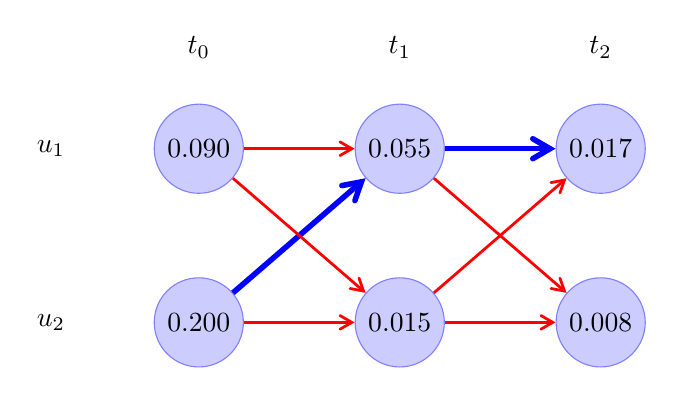
\begin{tikzpicture}
				\matrix[%
				matrix of math nodes,
				nodes={state},
				column sep=4em, row sep=7ex,
				] (s) {%
					{0.090} & {0.055} & {0.017}  \\
					{0.200} & {0.015} & {0.008}  \\
				};
				\node[above =3ex of s-1-1] {$t_{0}$};
				\node[above =3ex of s-1-2] {$t_{1}$};
				\node[above =3ex of s-1-3] {$t_{2}$};
				
				\node[left = of s-1-1, black] {$u_1$};
				\node[left = of s-2-1, black] {$u_2$};
			
				\draw[redthick] (s-1-1) -- node[above, black, 
				font=\scriptsize] 
				{$$} (s-1-2);
				\draw[bluethick] (s-2-1) -- node[above, black, 
				font=\scriptsize] 
				{$$} (s-1-2);
				\draw[bluethick] (s-1-2) -- node[above, black, 
				font=\scriptsize] 
				{$$} (s-1-3);
				\draw[redthick] (s-2-2) -- node[above, black, 
				font=\scriptsize] 
				{$$} (s-1-3);
				
				\draw[redthick] (s-2-1) -- node[above, black, 
				font=\scriptsize] 
				{$$} (s-2-2);
				\draw[redthick] (s-1-1) -- node[above, black, 
				font=\scriptsize] 
				{$$} (s-2-2);
				\draw[redthick] (s-2-2) -- node[above, black, 
				font=\scriptsize] 
				{$$} (s-2-3);
				\draw[redthick] (s-1-2) -- node[above, black, 
				font=\scriptsize] 
				{$$} (s-2-3);
				\end{tikzpicture}
				\captionof{figure}{Trellis of the most probable path.}
				\label{tab:trallis}
			\end{figure}
	Given $\delta_2$, $u_1$ is chosen since is the state with the maximum 
	value. Backtracking to $\delta_1$, $u_1$ is the state with the maximum 
	value and than, back to $\delta_0$, $u_2$ is the state with the maximum 
	value.

	Hence, the most probable sequence of states is $u_2, u_1, u_1$.
	
	
	\end{itemize}
}

	\Problem{
Implement a Python function \texttt{state\_probability(pi, A, s, t)} that takes 
initial state distribution $\pi$, transition matrix $A$, state $s$ and time $t$ 
and outputs the probability of state $s$ at time $t$. You can assume that the 
set of state is $S=\{0,1,\dots,N-1\}$. \\
You can use file \texttt{ex3.py} provided online.
}

\Solution{
	
	\begin{python}
import numpy as np

def state_probability(pi, A, s, T):
	prob = np.array(pi)
	for i in range(T):
		prob = np.matmul(prob, A)
	return prob[s]
	\end{python}


	
}
	\Problem{
	You are given three data points $(x, y) : (-1, 0), (0, 1), (1, 0)$. We are
	using squared error loss function 
	$\ell(y, \hat y) = (y - \hat y)^2$.
	
	\begin{itemize}
		\item[(a)] What is leave-one-out cross-validation error of constant 
		model $f(x) = c$?
		\item[(b)] What is leave-one-out cross-validation error of linear model 
		$f(x) = ax + b$?
	\end{itemize}
}

\Solution{
	\begin{itemize}
		\item[(a)] 
		Train set loss:
		
		\begin{align*}
			l_1(c) & = \min_c \big((0-c)^2 + (1-c)^2\big) = \min_c \big(c^2 -2c 
			+ 1 +c^2 \big) = \min_c \big( 2c^2 -2c +1 \big) =\dots \\
			l_2(c) & = \min_c \big((0-c)^2 + (0-c)^2\big) = \min_c \big(c^2 
			-c^2\big) = \min_c \big(0 \big)  = 0 \\
			l_3(c) & = \min_c \big((1-c)^2 + (0-c)^2\big) = \min_c \big(c^2 -2c 
			+1 +c^2\big) = \min_c \big(2c^2 -2c +1 \big) = \dots
		\end{align*}
		
		\begin{align*}
		l_1(c) = \frac{\partial l_1}{\partial c} &= 4c -2 = \frac{1}{2} \\
		l_3(c) = \frac{\partial l_3}{\partial c} &= 4c -2 = \frac{1}{2}
		\end{align*}
		
		
		Validation set loss:
		\begin{align*}
		e_1(c) &=  \big(0-l_1(c)\big)^2 =  \big(0-\frac{1}{2}\big)^2 = 
		\frac{1}{4} \\
		e_2(c) &=  \big(0-l_2(c)\big)^2 =  \big(1 - 0 \big)^2 = 1 \\
		e_3(c) &=  \big(0-l_3(c)\big)^2 =  \big(0 - \frac{1}{2} \big)^2 = 
		\frac{1}{4}
		\end{align*}
		
		
		$E=\frac{e_1+e_2+e_3}{3}=\frac{1}{2}$
		
		\item[(b)] 
	\end{itemize}
}

\end{document}
